\documentclass[spanish,notitlepage,letterpaper, 12pt]{article} % para articulo en castellano
\usepackage[ansinew]{inputenc} % Acepta caracteres en castellano
\usepackage[spanish]{babel} % silabea palabras castellanas
\usepackage{url}
\usepackage{amsmath}
\usepackage{amsfonts}
\usepackage{float}
\usepackage{amssymb}
\usepackage[colorlinks=true,urlcolor=blue,linkcolor=blue]{hyperref} % navega por el doc
\usepackage{graphicx}
\usepackage{geometry}      % See geometry.pdf to learn the layout options.
\geometry{letterpaper}                   % ... or a4paper or a5paper or ...
%\geometry{landscape}                % Activate for for rotated page geometry
%\usepackage[parfill]{parskip}    % Activate to begin paragraphs with an empty line rather than an indent
\usepackage{epstopdf}
\usepackage{fancyhdr} % encabezados y pies de pg
\usepackage{pgf,pgfarrows,pgfnodes}
\usepackage{graphicx}

\renewcommand{\spanishtablename}{Cuadro}

\pagestyle{fancy}
\chead{\bfseries Tarea 2}
\lhead{} % si se omite coloca el nombre de la seccion
\rhead{ }
\lfoot{\it }
\cfoot{}
\rfoot{\thepage}

\voffset = -0.25in
\textheight = 9.0in
\textwidth = 6.5in
\oddsidemargin = 0.in
\headheight = 20pt
\headwidth = 6.5in
\renewcommand{\headrulewidth}{0.5pt}
\renewcommand{\footrulewidth}{0,5pt}
\DeclareGraphicsRule{.tif}{png}{.png}{`convert #1 `dirname #1`/`basename #1 .tif`.png}

\begin{document}
\title{Tarea 2 \\ Análisis de texto}

\author{
\textbf{Erick Cervantes Mendieta} \\
\vspace{0.5cm}
\textnormal{Matrícula: 2032430}\\
\textit{Modelos Probabilistas Aplicados}}
\date{Septiembre 2020}

\maketitle

%------------------------------------------------

\section{Presentación de los datos}

Para esta tarea se analizó el libro titulado ``The Singing Mouse Stories", el cual se encuentra disponible de manera gratuita en el sitio Web: \emph{Project Gutenberg} \cite{Mouse}. Se utilizaron algunas técnicas para análisis de texto, como lo es las frecuencias de las letras y de las palabras, ideal para identificar rápidamente los temas comunes, y por otra parte, el agrupamiento de palabras, ya que a veces un grupo de palabras puede proporcionar una mejor perspectiva que una sola palabra.\\

En el cuadro \ref{t1} se pueden observar las cinco letras más utilizadas en el libro y en el cuadro \ref{t2}, se pueden observar las palabras más frecuentes en el texto.

\begin{table}[]
\centering
\caption{Letras más utilizadas en el libro}
\vspace{0.3 cm}
\begin{tabular}{c|c}
 Letra & Frecuencia \\
 \hline
  e & 10395 \\
  t & 7894 \\
  a & 6741 \\
  o & 6306 \\
  n & 5857 \\
\end{tabular}
\label{t1}
\end{table}

\begin{table}[]
\centering
\caption{Palabras más utilizadas en el libro}
\vspace{0.3 cm}
\begin{tabular}{c|c}
 Letra & Frecuencia \\
 \hline
  the & 1775 \\
  and & 895 \\
  of & 731 \\
  in & 367 \\
  it & 350 \\
\end{tabular}
\label{t2}
\end{table}

\section{Análisis de los datos}

Tanto las palabras como las letras utilizadas en la redacción del libro fueron analizadas, en el sentido de que se pudieron ordenaran según la frecuencia con la que aparecieron, por otra parte, los dígitos como las preposiciones, los artículos y las conjunciones fueron excluidos(as) del análisis, ya que estos no aportaban gran información.\\

La figura \ref{f1} muestra el número de veces que fueron utilizadas las letras del abecedario en el texto en orden descendente, en donde se puede  observar que la letra más utilizada fue la \textbf{e} y la menos utilizada fue la \textbf{x}. \\

\begin{figure}[]
\begin{center}
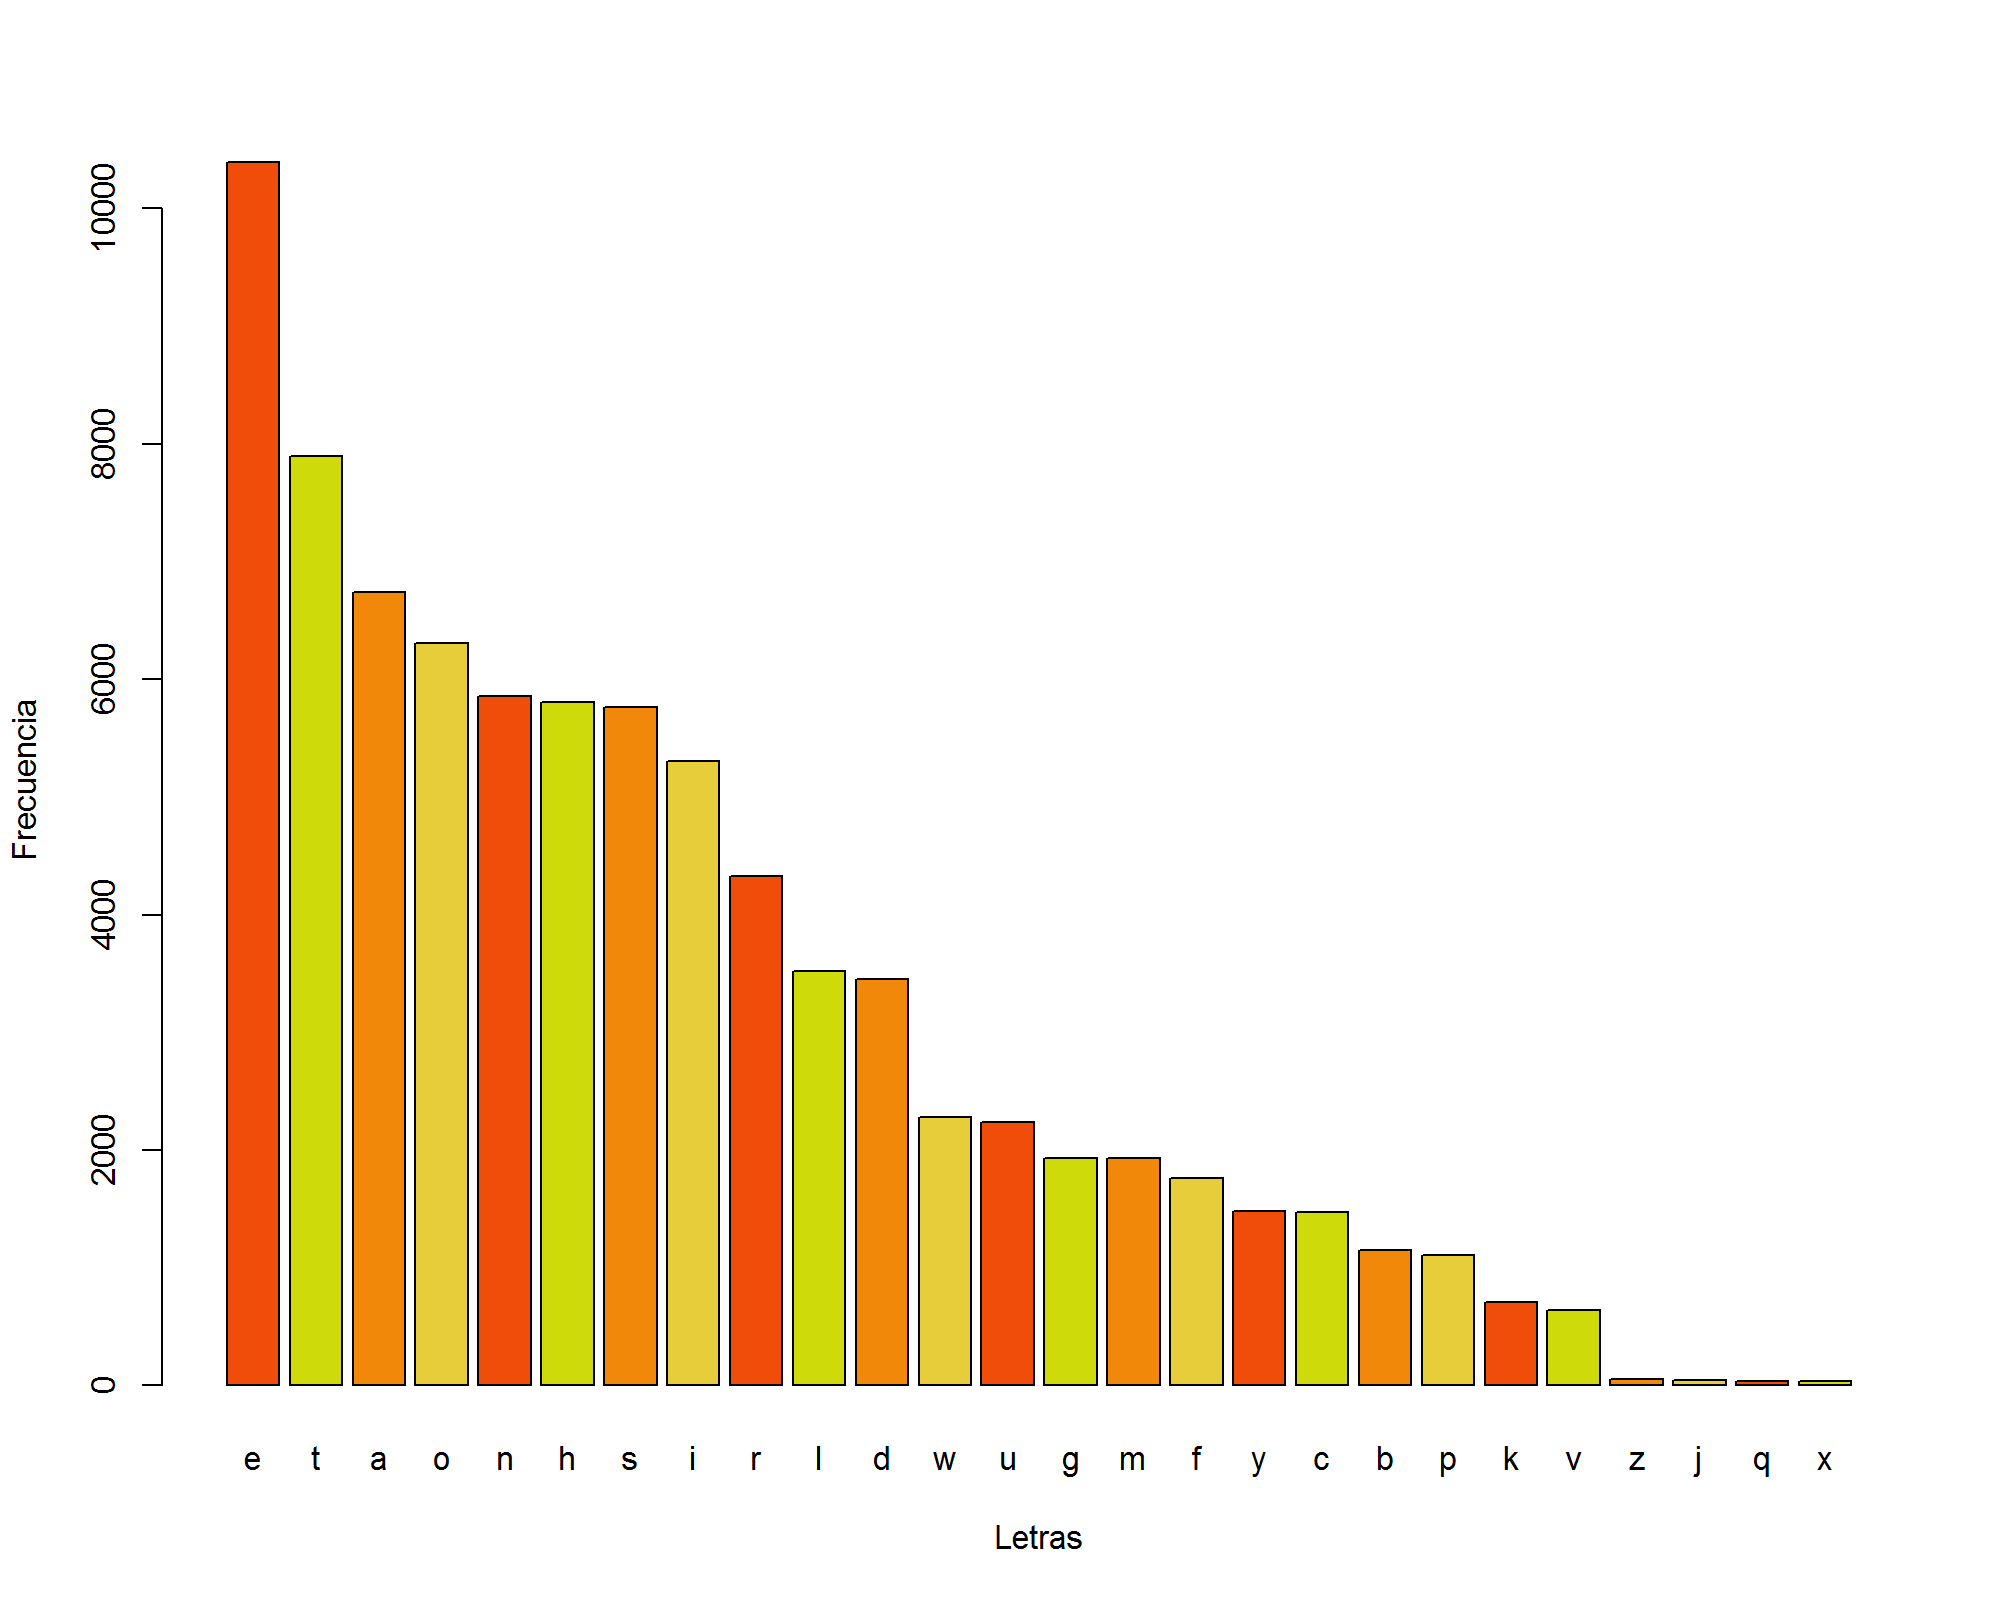
\includegraphics[width=16 cm]{FigModeloReporte/T2_letras.png}
\caption{Frecuencia de las letras utilizadas en el texto}\label{f1}
\end{center}
\end{figure}

En la figura \ref{f2} se pueden visualizar las palabras cuya frecuencia es mayor a cien, es decir, estas palabras aparecieron más de cien veces en el texto del libro, el listado es pequeño debido al tamaño del texto. Se observa que la palabra más utilizada fue el artículo \textbf{the}, seguida de la conjunción \textbf{and}, y en tercer lugar la preposición \textbf{of}, estas palabras son conocidas como \emph{palabras huecas} \cite{mendoza2018}, ya que aportan poca información semántica. Afortunadamente el programa R (Versión 4.0.2) \cite{LenguajeR} nos ofrece una herramienta para eliminar este tipo de palabras, lo que me permitió poder obtener bigramas para poder extraer información relevante del texto.\\

\begin{figure}[]
\begin{center}
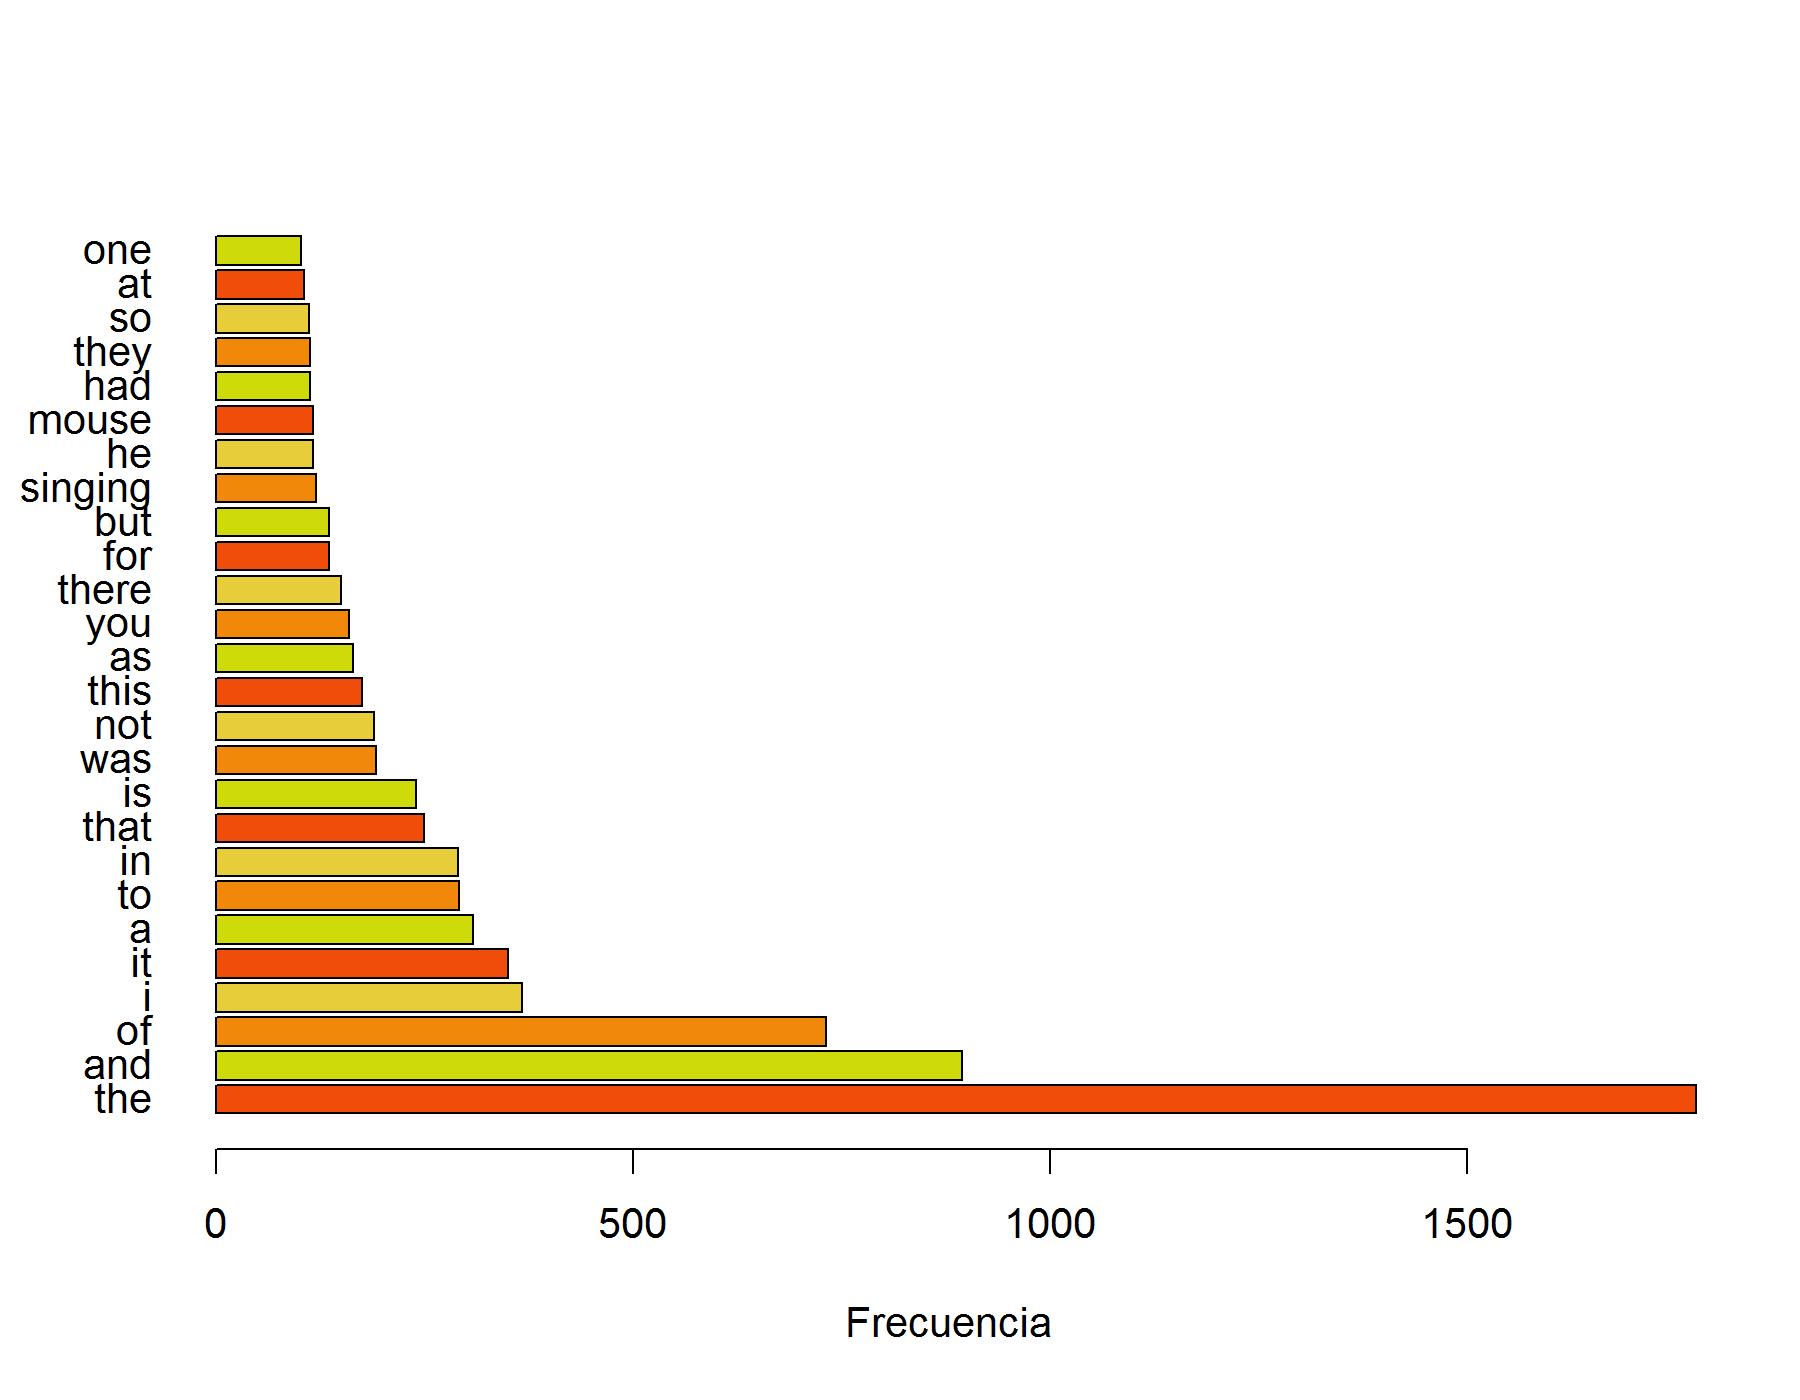
\includegraphics[width=16 cm]{FigModeloReporte/T2_palabras.png}
\caption{Frecuencia de las palabras más utilizadas en el texto}\label{f2}
\end{center}
\end{figure}

La figura \ref{f3} expone una red semántica con los bigrama obtenidos, los cuales no contienen palabras huecas. Esta red muestra la intensidad con la que se relacionan las palabras, es decir, la frecuencia con la que parejas de palabras aparecen en el texto. De dicha figura, podemos observar que aparece la palabra \emph{singing mouse}, lo que no da la referencia al personaje principal (debido al título también), otro conjunto de palabras que me llamó la atención fue \emph{lake belle marie}, por lo que supongo la historia se desarrolla cerca de un lago. Así mismo, \emph{little river} y \emph{delectable mountains} nos hacen sospechar, que la historia se desarrolla cerca de un paisaje lleno de naturaleza.

\begin{figure}[]
\begin{center}
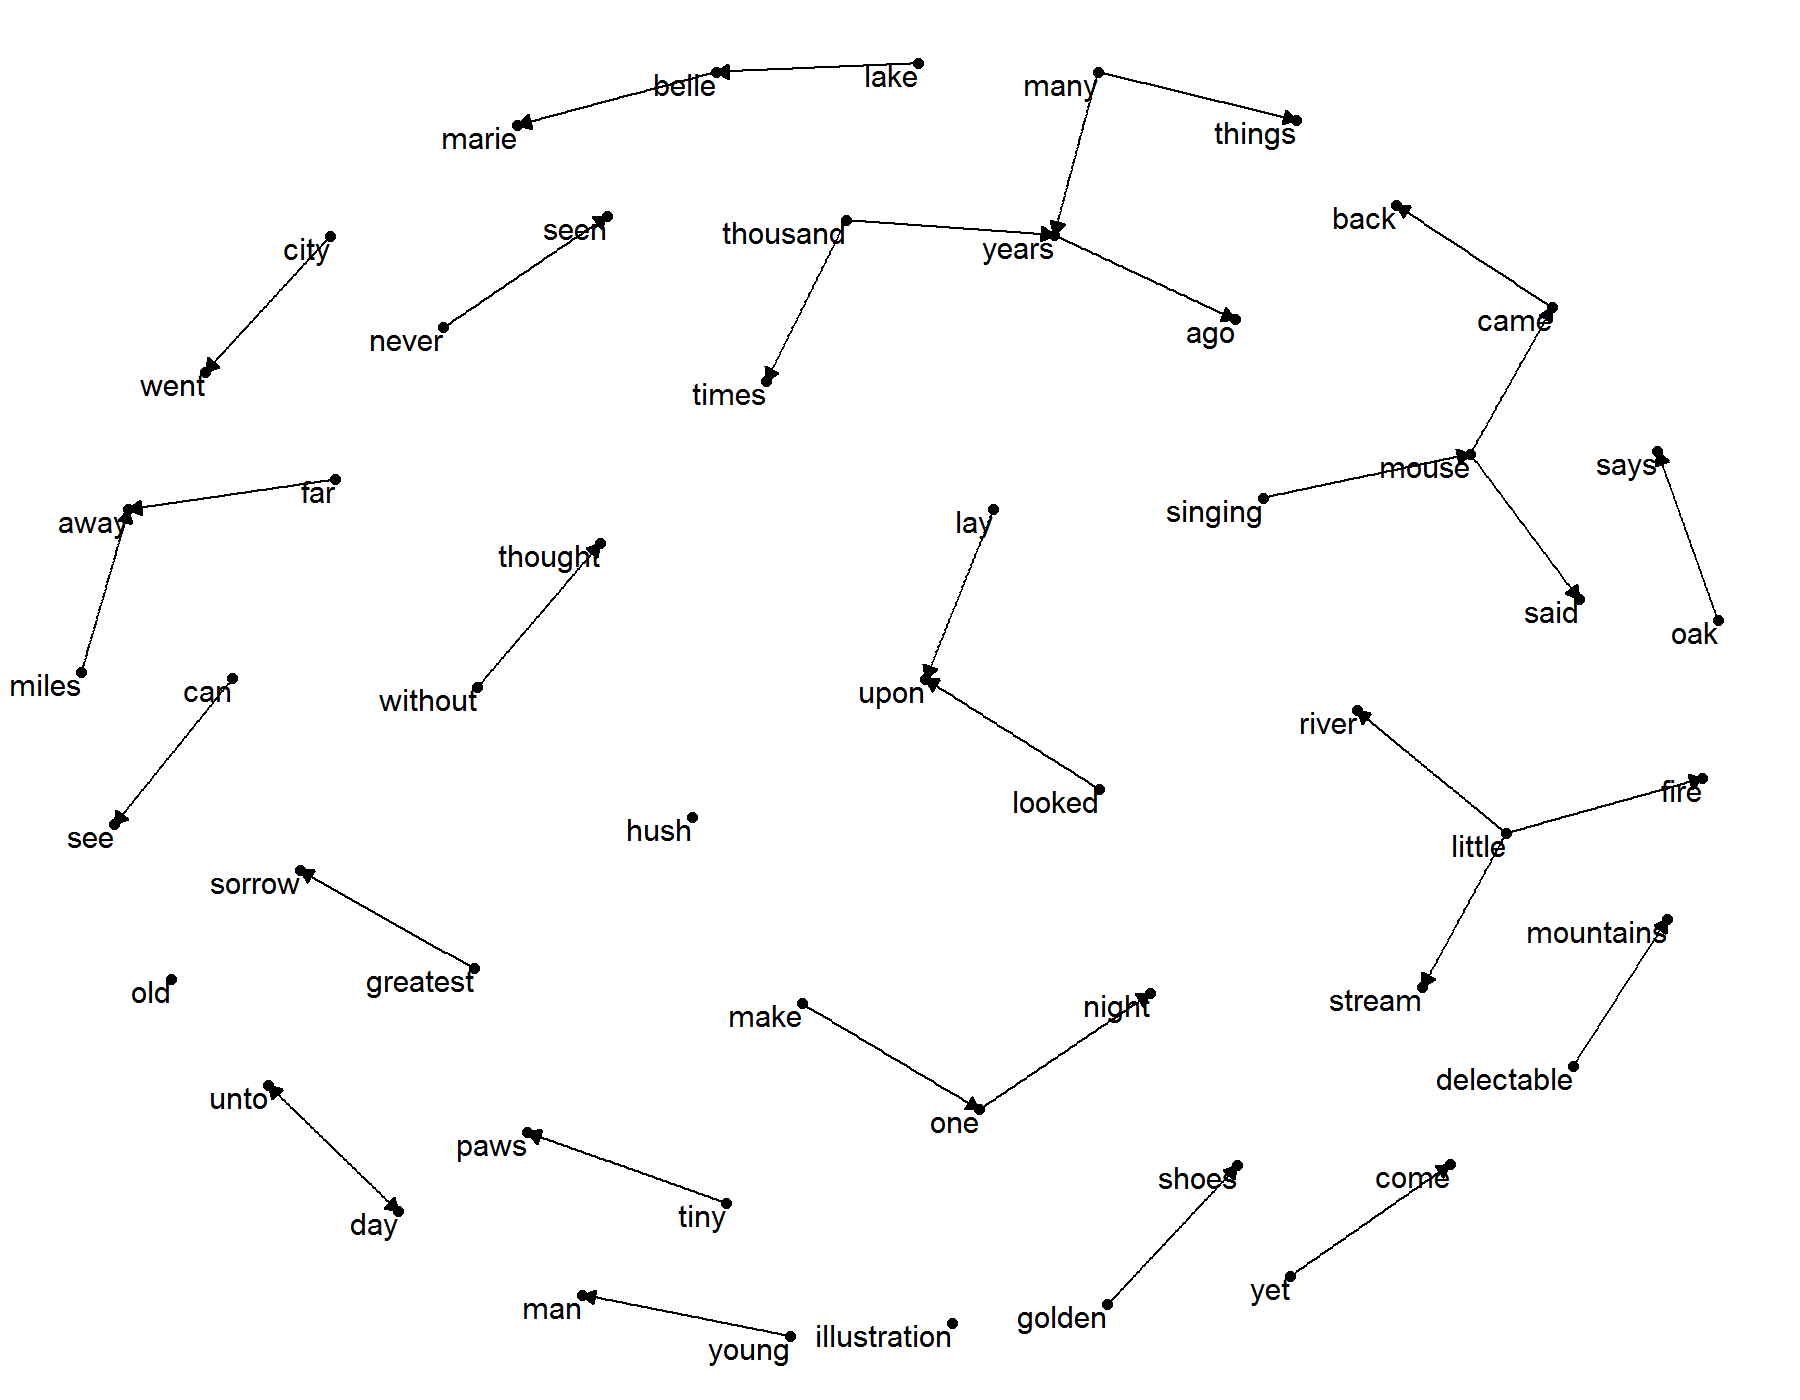
\includegraphics[width=16 cm]{FigModeloReporte/T2_bigrama.png}
\caption{Red semántica de parejas de palabras utilizadas en el texto}\label{f3}
\end{center}
\end{figure}

\bibliographystyle{plain}
\bibliography{BiblioE}

\end{document} 
